\section{Experimental evaluation}
\label{sec:exp}

In this section we present our experimental evaluation.  Our emphasis is to
compare the performance of \alggreedy and \algiterative, as well as to compare
the results with \algrolx~\cite{henderson2012rolx}.\footnote{We use an implementation by Circulo project, \url{https://github.com/lab41/circulo}.}
All datasets and software used in the experimental evaluation
will become publicly available.\footnote{{\sc url} not provided for blind review.}

%[[77, 14, 0], [6, 7, 1], [6, 12, 9]]

\spara{Experimental setup:}
We use 10 graphs of different sizes and densities, described in Table~\ref{table:datasets}.
The first three datasets, \karate, \dolphins, and \lesmis are obtained from UCIrvine Network Data
Repository.\footnote{\url{http://networkdata.ics.uci.edu/index.php}}
We create a synthetic dataset, \synth, with 3 groups of vertices, say $V_1$,
$V_2$, $V_3$, with $\abs{V_1} = 40$ and $\abs{V_2} = \abs{V_3} = 30$. 
We connect $V_1$ and $V_3$ to $V_2$ and fully connect $V_3$. After this
we apply noise by adding or removing an edge with a probability $p$. We vary $p$ from $0$ to $0.5$.
We also consider a collaboration network within a research
institute;\footnote{Name suppressed for blind review.} we add an edge
between the researchers if they have a joint paper in DBLP.
The
remaining datasets are obtained from Standford SNAP
Repository.\footnote{\url{http://snap.stanford.edu/data}}
\iffalse
\begin{itemize}
\item {\karate:} a social network of friendships between members of karate club at a US university in 1970.
\item {\dolphins:}  a social network of frequent associations between dolphins in a community living off Doubtful Sound in New Zealand.
\item {\lesmis:} co-appearance of characters in Les Miserables novel by Victor Hugo.
\item {\facebook:} friends list of Facebook users.
\item {\enron:} an e-mail communication network by Enron employees.
\item {\EUall:} an e-mail network from a EU research institution.
\item {\dblp:} a co-authorship network among computer science researchers.
\item {\youtube:} Youtube users network.
\end{itemize}
\fi

\begin{table}[th!]
\centering
\caption{Basic characteristics of the datasets. The second last column depicts the number of unique vertex degrees, the last column depicts the average degree.}
\begin{tabular*}{\columnwidth}{@{\extracolsep{\fill}}l r r r r r}
\toprule
Name&dir.&$\abs{V}$&$\abs{E}$& $\#\,\dg{}$ & $\overline{\dg{}}$\\
\midrule
{\karate} & no & 34 & 78 & 11 & 4.59 \\
{\dolphins} & no & 62 & 159 & 12 & 5.13 \\
{\lesmis} & no & 77 & 254 & 18&6.59 \\
{\facebook} & no & 4\,039 & 88\,234 & 227&43.69 \\
{\enron} & no & 36\,692 & 183\,831 & 334&10.02 \\
{\EUall} & yes & 265\,214 & 420\,045 & 311 &3.17\\
{\dblp} & no & 317\,080 & 1\,049\,866 & 199&6.62 \\
{\youtube} & no & 1\,134\,890 & 2\,987\,624 & 978&5.27 \\
{\synth} & no & 100 & 3270 & 2 & 32.70 \\
{\collab} & no & 132  & 237  & 14 & 3.59 \\
\bottomrule
\end{tabular*}
\label{table:datasets}
\end{table}

For each dataset, except for \synth and \collab,
we apply \algperfect, \alggreedy, and \algiterative. 
%\!\footnote{The code is available at \url{http://research.ics.aalto.fi/dmg/roles.zip}.}
For the 3 smallest graphs, we mine $k = 4$ roles.
For the remaining graphs, we set $k = 10$ roles.
When applying \alggreedy, we need to provide a role assignment as a seed. 
We consider 4 different variants:
($i$) \alginitone, every vertex is assigned the same role,
($ii$) \alginitdeg, vertices are sorted based on degree, and split into equal-size clusters,
($iii$) \alginitrnd, roles are assigned randomly, 
($iv$) \alginitkm, where we use the assignment given by \algiterative. 
The experiments conducted on \synth and \collab are described in the next section.

To speed-up the computation of \alggreedy, we implement the following
heuristic: if the role of a vertex has not changed during the 3 last iterations,
we no longer test the vertex. However, when we have converged, we start all over
by testing every vertex again. We stop, when no gain is possible, even if we consider every vertex.

\spara{Synthetic data:}
Our first step is to study how well we can discover the underlying structure in
\synth, the synthetic data.  In Figure~\ref{fig:synth}, we plot the 
adjusted Rand index for each method as a function of noise level.  
The shown numbers are averages over 100 repetitions. 
As expected the Rand index generally decreases
as the noise level increases: at $p = 0.5$, the graph is completely random
and there is no structure left to discover.
\alginitdeg, \alginitkm, and \algkm clearly outperfoms \alginitone and \alginitrnd, 
this implies that a good starting point is required for \alggreedy.
Interestingly, \algkm performs worse with small levels of noise but outperforms
\alggreedy variants once the noise level increase.


\begin{figure}
\begin{tikzpicture}
\begin{axis}[xlabel={noise level}, ylabel= {adjusted Rand index},
    height = 3.5cm,
    width = 8cm,
    cycle list name=yaf,
	yticklabel style={/pgf/number format/fixed},
	scaled ticks = false,
    xmin = 0,
    xmax = 0.5,
    ymax = 1,
	ymin = 0.0,
	%ytick = {0.02, 0.04, 0.06, 0.08, 0.1},
    xtick = {0.0, 0.1, 0.2, 0.3, 0.4, 0.5},
	legend entries = {\alginitdeg, \alginitkm, \algkm, \alginitone, \alginitrnd}, % \alginitkm, \algkm},
	legend pos = {outer north east},
	legend columns = 1
    ]

\addplot+[no markers]
    table[x index = 0, y index = 1, header = false]  {synth.dat};
\addplot+[no markers]
    table[x index = 0, y index = 5, header = false]  {synth.dat};
\addplot+[no markers]
    table[x index = 0, y index = 2, header = false]  {synth.dat};
\addplot+[no markers]
    table[x index = 0, y index = 3, header = false]  {synth.dat};
\addplot+[no markers]
    table[x index = 0, y index = 4, header = false]  {synth.dat};

\pgfplotsextra{\yafdrawaxis{0}{0.5}{0.00}{1}}
\end{axis}
\end{tikzpicture}
\caption{Adjusted Rand index between different methods and the ground truth as
a function of noise for the synthetic dataset. Larger numbers indicate stronger agreement.}
\label{fig:synth}
\end{figure}


\spara{Perfect assignments:}
Next, we consider the assignments given by \algperfect, given in Table~\ref{table:exact}. 

\begin{table}[htb!]
\centering
\caption{Role assignments discovered by \algperfect. $k$ stands for the number of discovered roles while
$\#\,\dg{}$ stands for the number of distinct degrees.}
\begin{tabular*}{\columnwidth}{@{\extracolsep{\fill}}l r r r r r}
\toprule
Name& $k$ & iter. & time & $\nicefrac{k}{\abs{V}}$ & $\nicefrac{k}{\#\,\dg{}}$ \\ 
\midrule
{\karate} &  27 & 2 & 1ms & 0.79 & 2.45 \\
{\dolphins} & 60 & 3 & 2ms & 0.96 & 5 \\
{\lesmis} & 56 & 5 & 4ms & 0.73& 3.11 \\
{\facebook} & 3\,872 & 5 & 0.9s & 0.96 & 17.06 \\
{\enron} & 20\,618 & 23 & 11s & 0.56 & 61.73 \\
{\EUall} & 20\,138 & 4 & 9s & 0.08 & 64.76 \\
{\dblp} & 233\,466 & 6 & 1m4s & 0.74 & 1173.2 \\
{\youtube} & 684\,010 & 7 & 3m47s & 0.61 & 699.39 \\
\bottomrule
\end{tabular*}
\label{table:exact}
\end{table}

We see that the number of roles needed to obtain a perfect solution is
typically large: with the exception of \EUall, we need at least half of the
number of vertices. The number of roles is higher than the number of unique
degrees, and the ratio increases for large graphs; these graphs have more ways
of forcing vertices to have unique roles.
The algorithm is practical even for large graphs as the
computational complexity $\bigO{n m \log n}$ given by Proposition~\ref{prop:exacttime} is fairly pessimistic:
only few iterations are needed for convergence, 
and each iteration requires only $\bigO{m \log n}$ time.

\spara{Performance of greedy and iterative algorithms:}
Our next step is to compare the performance of \alggreedy and \algiterative.
In Table~\ref{table:score}
we present the costs obtained by each algorithm, normalized
by the cost of a trivial role assignment, where each vertex is assigned
the same role.

\begin{table}[ht!]
\centering
\caption{Costs of role assignments, normalized by $\cost{\role'}$, where $\role'(v) = 0$ for every $v$.
Lower values are better.
The parameter $k$ stands for the number of roles. \algkm depicts \algiterative, while the remaining columns
depicts \alggreedy with different initializations.}
\begin{tabular*}{\columnwidth}{@{\extracolsep{\fill}}l r@{\hspace{6mm}}r@{\hspace{6mm}}r r r r} 
\toprule
Name& $k$ & \algkm & \alginitdeg & \alginitone & \alginitrnd & \alginitkm \\ 
\midrule
{\karate} &4&  0.103 & 0.097 & 0.141 & 0.125&0.089 \\
{\dolphins} &4& 0.306 & 0.253 & 0.219 & 0.255&0.213 \\
{\lesmis} &4& 0.142 & 0.124 & 0.121 & 0.133&0.118 \\
{\facebook} &10& 0.056 & 0.043 & 0.043 & 0.043&0.039 \\
{\enron} &10& 0.064 & 0.021 & 0.019 & 0.019&0.019 \\
{\EUall} &10& 0.097 & 0.029 & 0.024 & 0.035&0.028 \\
{\dblp} &10& 0.178 & 0.059  & 0.065 & 0.059&0.054 \\
{\youtube} &10& 0.202 & 0.029  & 0.029 & 0.029&0.029 \\
\bottomrule
\end{tabular*}
\label{table:score}
\end{table}

We see that the best scores are obtained by \alginitkm, that is, \alggreedy
initialized by \algiterative. Curiously enough, \algiterative alone performs
the worst. These results hint that the search space is highly non-trivial,
containing a plethora of local minima. This is further supported by Table~\ref{table:randgreedy},
where we report adjusted Rand index.\footnote{Value 1 corresponds to a complete agreement, 
while 0 implies that the assignments are independent.}
The index implies that while the obtained results all correlate positively they do differ.
This puts extra emphasis on a good initialization of \alggreedy.

\begin{table}[thb!]

\caption{Adjusted Rand indices between different initializations of \alggreedy. }
\setlength{\tabcolsep}{0pt}
\begin{tabular*}{\columnwidth}{@{\extracolsep{\fill}}l r r r r r r} 
\toprule
%Name & \textsc{D}-\textsc{O}&\textsc{D}-\textsc{RD}&\textsc{D}-\textsc{KG}&\textsc{O}-\textsc{RD}&\textsc{O}-\textsc{KG}&\textsc{RD}-\textsc{KG}  \\ 
Name &
$\nicefrac{\alginitdeg}{\alginitone}$ &
$\nicefrac{\alginitdeg}{\alginitrnd}$ &
$\nicefrac{\alginitdeg}{\alginitkm}$ &
$\nicefrac{\alginitone}{\alginitrnd}$ &
$\nicefrac{\alginitone}{\alginitkm}$ &
$\nicefrac{\alginitrnd}{\alginitkm}$ \\


\midrule
{\karate}  &0.104&0.116&0.485&0.107&0.105&0.222 \\
{\dolphins}&0.419&0.134&0.441&0.181&0.374&0.163  \\
{\lesmis}  &0.437&0.449&0.453&0.192&0.603&0.283 \\
{\facebook}&0.389&0.385&0.356&0.591&0.521&0.535  \\
{\enron}   &0.224&0.135&0.301&0.157&0.232&0.135  \\
{\EUall}   &0.421&0.272&0.282&0.305&0.365&0.218\\
{\dblp}    &0.291&0.411&0.427&0.226&0.219&0.307\\
\bottomrule
\end{tabular*}
\label{table:randgreedy}
\end{table}

The left plot in Figure~\ref{fig:facebook} shows the cost as a function of $k$
for \facebook dataset.  Naturally, the cost decreases as we increase $k$. The
change is more rapid for small values of $k$, and evens out for large values.

Let us now study how well the role assignment correlates with vertex degree.  
Since the
roles are symbolic, we sort the roles based on average degree, and compared
the roles and degrees using Kendall-$\tau$.\footnote{We use the $b$ variant
to accommodate the ties.} We see from the results given in
Table~\ref{table:kendaltau} that there is significant correlation between the
degrees and the role assignment. Naturally, this is partly due to how we sort
the roles.  However, there are some subtle differences. The coefficients depend
on the dataset, for example, \EUall obtains one of the lowest values. There is
a clear difference between \algiterative and \alggreedy: the former producing
ranks with weak or almost no correlation with the degree. This advances further
the notion that \algiterative gets stuck in local minimum, and should not be used
alone.

\begin{table}[htb!]
\centering
%\caption{Kendall-$\tau$ statistics between degree-based ranking and role-based ranking. Role-based ranking is implemented by our algorithms with different initialization. \textsc{deg} for degree based initial role assignment, \textsc{one} for assigning one role for all node during initialization, \textsc{rnd} for assigning random roles, and \textsc{i+g} for k-means based initialization.}

\caption{Kendall-$\tau$ statistics between role assignments and vertex degree.
Roles are sorted based on their average degree.
\algkm depicts \algiterative, while the remaining columns
depicts \alggreedy with different initializations.
}

\begin{tabular*}{\columnwidth}{@{\extracolsep{\fill}}l r r r r r}
\toprule
Name& \algkm & \alginitdeg & \alginitone & \alginitrnd & \alginitkm \\ 
\midrule
{\karate}   &0.449 &0.794 &0.501 & 0.636&0.636 \\
{\dolphins} &0.123 &0.661 &0.672 & 0.598&0.744 \\
{\lesmis}   &0.228 &0.711 &0.729 & 0.679&0.734 \\
{\facebook} &0.052 &0.707 &0.714 & 0.741&0.739 \\
{\enron}    &0.007 &0.467 &0.474 & 0.459&0.467 \\
{\EUall}    &0.003 &0.327 &0.203 & 0.275&0.352 \\
{\dblp}     &0.008 &0.596 &0.559 & 0.564&0.536 \\
{\youtube}  &0.004 &0.467 &0.454 & 0.404&0.465  \\
\bottomrule
\end{tabular*}

\label{table:kendaltau}
\end{table}



\spara{Running time:}
Let us now consider the computational complexity of the algorithms.  We present the
number of iterations needed for convergence in Table~\ref{table:iterations},
and the running times in Table~\ref{table:time}. The number of required
iterations is modest, especially when compared to the size of the input graph.
The running times are manageable: we should point out that we implemented
\alggreedy using Python, an implementation with a more efficient programming
platform should make the algorithm more user-friendly, especially for large
graphs. As expected, the running times increase as we increase the number of roles; 
see the right plot in Figure~\ref{fig:facebook}.


\begin{table}[htb!]
\centering
\caption{Total number of iterations required for convergence.
\algkm depicts \algiterative, while the remaining columns
depicts \alggreedy with different initializations.
}

\begin{tabular*}{\columnwidth}{@{\extracolsep{\fill}}l r r r r r}
\toprule
Name& \algkm & \alginitdeg & \alginitone & \alginitrnd & \alginitkm \\ 
\midrule
{\karate}   &  2 & 2   & 5   & 15  & 5 \\
{\dolphins} &  2 & 3   & 5   & 12  & 5 \\
{\lesmis}   &  2 & 14  & 16  & 13  & 5 \\
{\facebook} &  2 & 85  & 92  & 131 & 73 \\
{\enron}    &  3 & 180 & 220 & 215 & 124 \\
{\EUall}    &  3 & 719 & 404 & 2921& 122 \\
{\dblp}     &  3 & 17  & 41  & 56  & 53 \\
{\youtube}  &  4 & 462 & 413 & 471 & 552 \\
\bottomrule
\end{tabular*}
\label{table:iterations}
\end{table}

\begin{table}[htb!]
\centering
\caption{Evaluation time of algorithms.
\algkm depicts \algiterative, while the remaining columns
depicts \alggreedy with different initializations.
}

\begin{tabular*}{\columnwidth}{@{\extracolsep{\fill}}l r r r r r}
 \toprule
Name& \algkm & \alginitdeg & \alginitone & \alginitrnd & \alginitkm \\ 
\midrule
{\karate}   &2ms  &5ms    &14ms   & 19ms   &14ms \\
{\dolphins} &4ms  &14ms   &22ms   & 32ms   &29ms \\
{\lesmis}   &5ms  &46ms   &48ms   & 29ms   &36ms \\
{\facebook} &0.4s &39s    &41s    & 53s    &39s \\
{\enron}    &1.9s &7m6s   &9m4s   & 9m5s   &7m40s \\
{\EUall}    &21s  &49m3s  & 21m4s & 1h45m  &10m22s \\
{\dblp}     &21s  &1h21m  &22m3s  & 41m6s  &29m57s \\
{\youtube}  & 87s &12h10m &7h30m  & 16h10m &14h52m  \\
\bottomrule
\end{tabular*}

\label{table:time}
\end{table}





\begin{figure}[htb!]
\begin{tikzpicture}
\begin{axis}[xlabel={number of roles $k$}, ylabel= {$\cost{\role} / \cost{\role'}$},
    height = 3.5cm,
    width = 0.52\columnwidth,
    cycle list name=yaf,
	yticklabel style={/pgf/number format/fixed},
	scaled ticks = false,
    %xmin = 1,
    %ymin = 0.2,
    ymax = 0.4,
	ymin = 0.0,
	%ytick = {0.02, 0.04, 0.06, 0.08, 0.1},
    xtick = {2, 8, 14, 20},
	legend entries = {\alginitdeg, \alginitone, \alginitrnd, \alginitkm, \algkm},
	legend columns = 2
    ]

\addplot+[no markers]
    table[x index = 0, y index = 1]  {images/plot data/varying_k_plot.txt};
\addplot+[no markers]
    table[x index = 0, y index = 2]  {images/plot data/varying_k_plot.txt};
\addplot+[no markers]
    table[x index = 0, y index = 3]  {images/plot data/varying_k_plot.txt};
\addplot+[no markers]
    table[x index = 0, y index = 8]  {images/plot data/varying_k_plot.txt};
\addplot+[no markers]
    table[x index = 0, y index = 7]  {images/plot data/varying_k_plot.txt};

\pgfplotsextra{\yafdrawaxis{2}{20}{0.00}{0.4}}
\end{axis}
\end{tikzpicture}\hspace{-2mm}
\begin{tikzpicture}
\begin{axis}[xlabel={number of roles $k$}, ylabel= {time (seconds)},
    height = 3.5cm,
    width = 0.52\columnwidth,
    cycle list name=yaf,
	yticklabel style={/pgf/number format/fixed},
	scaled ticks = false,
    ymax = 140,
	ymin = 0,
    xtick = {2, 8, 14, 20},
    ytick = {0, 35, 70, 105, 140},
	%legend entries = {\alginitdeg, \alginitone, \alginitrnd, \alginitkm, \algkm},
	%legend pos = {north west}
    ]

\addplot+[no markers]
    table[x index = 0, y index = 4]  {images/plot data/varying_k_plot.txt};
\addplot+[no markers]
    table[x index = 0, y index = 5]  {images/plot data/varying_k_plot.txt};
\addplot+[no markers]
    table[x index = 0, y index = 6]  {images/plot data/varying_k_plot.txt};
\addplot+[no markers]
    table[x index = 0, y index = 10]  {images/plot data/varying_k_plot.txt};
\addplot+[no markers]
    table[x index = 0, y index = 9]  {images/plot data/varying_k_plot.txt};

\pgfplotsextra{\yafdrawaxis{2}{20}{0}{140}}
\end{axis}
\end{tikzpicture}
\caption{The normalized cost and the execution time for \facebook dataset.
The cost is normalized by $\cost{r'}$ such that $r'(v) = 0$, for every $v$, that is, $r'$ assigns the same role to every vertex.}
\label{fig:facebook}
\end{figure}

\begin{figure}[ht!]
\pgfplotsset{every axis plot post/.append style= {line width=0.5pt}}
\begin{tikzpicture}
\begin{axis}[xlabel={$\role(v) = 1$\hspace{1.8cm}$\role(v) = 2$\hspace{1.8cm}$\role(v) = 3$}, ylabel= {profile of $v$},
    height = 3.5cm,
    width = 9cm,
    cycle list name=yaf,
	yticklabel style={/pgf/number format/fixed},
	scaled ticks = false,
	no markers,
    %xmin = 0,
    %xmax = 0.5,
    %ymax = 1,
	%ymin = 0.0,
	xtick = {0,1,...,8},
	xticklabels = {1, 2, 3, 1, 2, 3, 1, 2, 3},
    ]

\addplot+[no markers, yafcolor5, opacity=0.5] coordinates {(0.000000, 2.048693) (1.000000, 1.061855) (2.000000, 1.116127)};
\addplot+[no markers, yafcolor5, opacity=0.5] coordinates {(3.000000, 4.048591) (4.000000, 2.169080) (5.000000, 1.028571)};
\addplot+[no markers, yafcolor5, opacity=0.5] coordinates {(6.000000, 9.062049) (7.000000, 8.006494) (8.000000, 4.011036)};
\addplot+[no markers, yafcolor5, opacity=0.5] coordinates {(0.000000, 1.117320) (1.000000, 1.021851) (2.000000, 0.056325)};
\addplot+[no markers, yafcolor5, opacity=0.5] coordinates {(0.000000, 1.086392) (1.000000, 1.001058) (2.000000, 0.042479)};
\addplot+[no markers, yafcolor5, opacity=0.5] coordinates {(0.000000, 1.107793) (1.000000, 1.011542) (2.000000, 0.138227)};
\addplot+[no markers, yafcolor5, opacity=0.5] coordinates {(3.000000, 2.184133) (4.000000, 2.019709) (5.000000, 1.180901)};
\addplot+[no markers, yafcolor5, opacity=0.5] coordinates {(0.000000, 1.173462) (1.000000, 2.133685) (2.000000, 0.113891)};
\addplot+[no markers, yafcolor5, opacity=0.5] coordinates {(3.000000, 2.069210) (4.000000, 2.128067) (5.000000, 3.193795)};
\addplot+[no markers, yafcolor5, opacity=0.5] coordinates {(6.000000, 2.044037) (7.000000, 4.137985) (8.000000, 2.099409)};
\addplot+[no markers, yafcolor5, opacity=0.5] coordinates {(3.000000, 2.075520) (4.000000, 3.021034) (5.000000, 2.191576)};
\addplot+[no markers, yafcolor5, opacity=0.5] coordinates {(3.000000, 1.153470) (4.000000, 4.199740) (5.000000, 3.024490)};
\addplot+[no markers, yafcolor5, opacity=0.5] coordinates {(6.000000, 5.077312) (7.000000, 3.123517) (8.000000, 0.094952)};
\addplot+[no markers, yafcolor5, opacity=0.5] coordinates {(3.000000, 2.053608) (4.000000, 0.002512) (5.000000, 1.132655)};
\addplot+[no markers, yafcolor5, opacity=0.5] coordinates {(3.000000, 1.112364) (4.000000, 1.092448) (5.000000, 1.023804)};
\addplot+[no markers, yafcolor5, opacity=0.5] coordinates {(0.000000, 1.078327) (1.000000, 1.107323) (2.000000, 0.140481)};
\addplot+[no markers, yafcolor5, opacity=0.5] coordinates {(3.000000, 2.085827) (4.000000, 2.066651) (5.000000, 3.156963)};
\addplot+[no markers, yafcolor5, opacity=0.5] coordinates {(0.000000, 0.134948) (1.000000, 1.054494) (2.000000, 0.197251)};
\addplot+[no markers, yafcolor5, opacity=0.5] coordinates {(3.000000, 3.095833) (4.000000, 1.046950) (5.000000, 0.107700)};
\addplot+[no markers, yafcolor5, opacity=0.5] coordinates {(0.000000, 0.125660) (1.000000, 1.138250) (2.000000, 3.063673)};
\addplot+[no markers, yafcolor5, opacity=0.5] coordinates {(6.000000, 7.137089) (7.000000, 6.101174) (8.000000, 2.151246)};
\addplot+[no markers, yafcolor5, opacity=0.5] coordinates {(6.000000, 5.117427) (7.000000, 6.138516) (8.000000, 3.088857)};
\addplot+[no markers, yafcolor5, opacity=0.5] coordinates {(0.000000, 2.033055) (1.000000, 1.139311) (2.000000, 0.169768)};
\addplot+[no markers, yafcolor5, opacity=0.5] coordinates {(0.000000, 1.094012) (1.000000, 1.022381) (2.000000, 1.179402)};
\addplot+[no markers, yafcolor5, opacity=0.5] coordinates {(3.000000, 1.020000) (4.000000, 0.021330) (5.000000, 1.066672)};
\addplot+[no markers, yafcolor5, opacity=0.5] coordinates {(0.000000, 0.137323) (1.000000, 1.096929) (2.000000, 0.009710)};
\addplot+[no markers, yafcolor5, opacity=0.5] coordinates {(3.000000, 3.022224) (4.000000, 2.061665) (5.000000, 2.089961)};
\addplot+[no markers, yafcolor5, opacity=0.5] coordinates {(0.000000, 0.025161) (1.000000, 1.091831) (2.000000, 0.013726)};
\addplot+[no markers, yafcolor5, opacity=0.5] coordinates {(3.000000, 4.008384) (4.000000, 3.130698) (5.000000, 0.094461)};
\addplot+[no markers, yafcolor5, opacity=0.5] coordinates {(0.000000, 0.098773) (1.000000, 1.008217) (2.000000, 1.170646)};
\addplot+[no markers, yafcolor5, opacity=0.5] coordinates {(3.000000, 2.043718) (4.000000, 2.190553) (5.000000, 2.079254)};
\addplot+[no markers, yafcolor5, opacity=0.5] coordinates {(6.000000, 8.135348) (7.000000, 8.128556) (8.000000, 4.009503)};
\addplot+[no markers, yafcolor5, opacity=0.5] coordinates {(3.000000, 2.081297) (4.000000, 2.102641) (5.000000, 2.080386)};
\addplot+[no markers, yafcolor5, opacity=0.5] coordinates {(3.000000, 3.176335) (4.000000, 3.038267) (5.000000, 0.154644)};
\addplot+[no markers, yafcolor5, opacity=0.5] coordinates {(3.000000, 2.020044) (4.000000, 1.147269) (5.000000, 0.155289)};
\addplot+[no markers, yafcolor5, opacity=0.5] coordinates {(3.000000, 3.138915) (4.000000, 2.016678) (5.000000, 2.006777)};
\addplot+[no markers, yafcolor5, opacity=0.5] coordinates {(0.000000, 0.172347) (1.000000, 1.086429) (2.000000, 0.063491)};
\addplot+[no markers, yafcolor5, opacity=0.5] coordinates {(0.000000, 1.103550) (1.000000, 2.039287) (2.000000, 1.194756)};
\addplot+[no markers, yafcolor5, opacity=0.5] coordinates {(0.000000, 1.196697) (1.000000, 0.058902) (2.000000, 1.115331)};
\addplot+[no markers, yafcolor5, opacity=0.5] coordinates {(6.000000, 5.164358) (7.000000, 4.150825) (8.000000, 1.024417)};
\addplot+[no markers, yafcolor5, opacity=0.5] coordinates {(0.000000, 1.046079) (1.000000, 2.157204) (2.000000, 0.173362)};
\addplot+[no markers, yafcolor5, opacity=0.5] coordinates {(0.000000, 1.198987) (1.000000, 0.170441) (2.000000, 2.136931)};
\addplot+[no markers, yafcolor5, opacity=0.5] coordinates {(3.000000, 3.092172) (4.000000, 2.122341) (5.000000, 2.113979)};
\addplot+[no markers, yafcolor5, opacity=0.5] coordinates {(0.000000, 0.176572) (1.000000, 1.004209) (2.000000, 1.173608)};
\addplot+[no markers, yafcolor5, opacity=0.5] coordinates {(0.000000, 1.013635) (1.000000, 1.188082) (2.000000, 0.083876)};
\addplot+[no markers, yafcolor5, opacity=0.5] coordinates {(3.000000, 3.049745) (4.000000, 3.081481) (5.000000, 2.148040)};
\addplot+[no markers, yafcolor5, opacity=0.5] coordinates {(0.000000, 0.193047) (1.000000, 0.135428) (2.000000, 1.147229)};
\addplot+[no markers, yafcolor5, opacity=0.5] coordinates {(3.000000, 1.048478) (4.000000, 1.080664) (5.000000, 1.170653)};
\addplot+[no markers, yafcolor5, opacity=0.5] coordinates {(3.000000, 3.073167) (4.000000, 2.104199) (5.000000, 2.191317)};
\addplot+[no markers, yafcolor5, opacity=0.5] coordinates {(6.000000, 4.175555) (7.000000, 4.143335) (8.000000, 1.032033)};
\addplot+[no markers, yafcolor5, opacity=0.5] coordinates {(0.000000, 0.093893) (1.000000, 2.066804) (2.000000, 1.107506)};
\addplot+[no markers, yafcolor5, opacity=0.5] coordinates {(0.000000, 0.048099) (1.000000, 1.067497) (2.000000, 1.157753)};
\addplot+[no markers, yafcolor5, opacity=0.5] coordinates {(6.000000, 4.088359) (7.000000, 4.168893) (8.000000, 1.031132)};
\addplot+[no markers, yafcolor5, opacity=0.5] coordinates {(0.000000, 0.177103) (1.000000, 1.068921) (2.000000, 1.010135)};
\addplot+[no markers, yafcolor5, opacity=0.5] coordinates {(0.000000, 2.139463) (1.000000, 1.020948) (2.000000, 1.129520)};
\addplot+[no markers, yafcolor5, opacity=0.5] coordinates {(3.000000, 2.077707) (4.000000, 2.145405) (5.000000, 2.197926)};
\addplot+[no markers, yafcolor5, opacity=0.5] coordinates {(0.000000, 1.118861) (1.000000, 0.102623) (2.000000, 1.177357)};
\addplot+[no markers, yafcolor5, opacity=0.5] coordinates {(0.000000, 2.157458) (1.000000, 0.187501) (2.000000, 1.128455)};
\addplot+[no markers, yafcolor5, opacity=0.5] coordinates {(0.000000, 0.146163) (1.000000, 0.000764) (2.000000, 1.170119)};
\addplot+[no markers, yafcolor5, opacity=0.5] coordinates {(0.000000, 0.047204) (1.000000, 1.093094) (2.000000, 0.192402)};
\addplot+[no markers, yafcolor5, opacity=0.5] coordinates {(6.000000, 3.192990) (7.000000, 4.120409) (8.000000, 0.040005)};
\addplot+[no markers, yafcolor5, opacity=0.5] coordinates {(0.000000, 0.038705) (1.000000, 0.089108) (2.000000, 1.123949)};
\addplot+[no markers, yafcolor5, opacity=0.5] coordinates {(3.000000, 3.072217) (4.000000, 1.054186) (5.000000, 1.055189)};
\addplot+[no markers, yafcolor5, opacity=0.5] coordinates {(0.000000, 1.062288) (1.000000, 3.122484) (2.000000, 0.187300)};
\addplot+[no markers, yafcolor5, opacity=0.5] coordinates {(0.000000, 0.146127) (1.000000, 1.154901) (2.000000, 0.101090)};
\addplot+[no markers, yafcolor5, opacity=0.5] coordinates {(0.000000, 1.106124) (1.000000, 0.051915) (2.000000, 0.042402)};
\addplot+[no markers, yafcolor5, opacity=0.5] coordinates {(0.000000, 1.180414) (1.000000, 0.084543) (2.000000, 1.001060)};
\addplot+[no markers, yafcolor5, opacity=0.5] coordinates {(0.000000, 1.006890) (1.000000, 0.061349) (2.000000, 1.145317)};
\addplot+[no markers, yafcolor5, opacity=0.5] coordinates {(3.000000, 1.061495) (4.000000, 0.090228) (5.000000, 2.075995)};
\addplot+[no markers, yafcolor5, opacity=0.5] coordinates {(0.000000, 1.148371) (1.000000, 0.016729) (2.000000, 0.104673)};
\addplot+[no markers, yafcolor5, opacity=0.5] coordinates {(0.000000, 0.165232) (1.000000, 1.078190) (2.000000, 1.121461)};
\addplot+[no markers, yafcolor5, opacity=0.5] coordinates {(0.000000, 0.035062) (1.000000, 1.084556) (2.000000, 1.155710)};
\addplot+[no markers, yafcolor5, opacity=0.5] coordinates {(0.000000, 0.176530) (1.000000, 1.131280) (2.000000, 1.125604)};
\addplot+[no markers, yafcolor5, opacity=0.5] coordinates {(3.000000, 2.066116) (4.000000, 2.024263) (5.000000, 3.132250)};
\addplot+[no markers, yafcolor5, opacity=0.5] coordinates {(0.000000, 2.038127) (1.000000, 3.039589) (2.000000, 2.060896)};
\addplot+[no markers, yafcolor5, opacity=0.5] coordinates {(3.000000, 1.015559) (4.000000, 3.133453) (5.000000, 2.119783)};
\addplot+[no markers, yafcolor5, opacity=0.5] coordinates {(0.000000, 1.050512) (1.000000, 1.157838) (2.000000, 1.073797)};
\addplot+[no markers, yafcolor5, opacity=0.5] coordinates {(0.000000, 1.089656) (1.000000, 0.168609) (2.000000, 0.033592)};
\addplot+[no markers, yafcolor5, opacity=0.5] coordinates {(0.000000, 2.046502) (1.000000, 4.042532) (2.000000, 2.197783)};
\addplot+[no markers, yafcolor5, opacity=0.5] coordinates {(0.000000, 1.010084) (1.000000, 1.039419) (2.000000, 0.100716)};
\addplot+[no markers, yafcolor5, opacity=0.5] coordinates {(0.000000, 1.060785) (1.000000, 2.118499) (2.000000, 0.036714)};
\addplot+[no markers, yafcolor5, opacity=0.5] coordinates {(0.000000, 1.058419) (1.000000, 0.011756) (2.000000, 1.040483)};
\addplot+[no markers, yafcolor5, opacity=0.5] coordinates {(0.000000, 1.011121) (1.000000, 1.188173) (2.000000, 0.095689)};
\addplot+[no markers, yafcolor5, opacity=0.5] coordinates {(0.000000, 2.057616) (1.000000, 0.095931) (2.000000, 0.160947)};
\addplot+[no markers, yafcolor5, opacity=0.5] coordinates {(0.000000, 0.145101) (1.000000, 0.021632) (2.000000, 1.159654)};
\addplot+[no markers, yafcolor5, opacity=0.5] coordinates {(0.000000, 1.004373) (1.000000, 0.163021) (2.000000, 1.035474)};
\addplot+[no markers, yafcolor5, opacity=0.5] coordinates {(0.000000, 0.055133) (1.000000, 0.028147) (2.000000, 1.055101)};
\addplot+[no markers, yafcolor5, opacity=0.5] coordinates {(0.000000, 0.087688) (1.000000, 0.187955) (2.000000, 1.151000)};
\addplot+[no markers, yafcolor5, opacity=0.5] coordinates {(0.000000, 0.036763) (1.000000, 1.130515) (2.000000, 1.036827)};
\addplot+[no markers, yafcolor5, opacity=0.5] coordinates {(3.000000, 2.103869) (4.000000, 0.008756) (5.000000, 1.161992)};
\addplot+[no markers, yafcolor5, opacity=0.5] coordinates {(0.000000, 1.029638) (1.000000, 2.127924) (2.000000, 0.027319)};
\addplot+[no markers, yafcolor5, opacity=0.5] coordinates {(3.000000, 2.036497) (4.000000, 2.058487) (5.000000, 1.138129)};
\addplot+[no markers, yafcolor5, opacity=0.5] coordinates {(0.000000, 1.104150) (1.000000, 0.160857) (2.000000, 1.053830)};
\addplot+[no markers, yafcolor5, opacity=0.5] coordinates {(0.000000, 1.021757) (1.000000, 0.012717) (2.000000, 0.026793)};
\addplot+[no markers, yafcolor5, opacity=0.5] coordinates {(0.000000, 0.119912) (1.000000, 0.021691) (2.000000, 1.010647)};
\addplot+[no markers, yafcolor5, opacity=0.5] coordinates {(0.000000, 1.095701) (1.000000, 1.166578) (2.000000, 1.049193)};
\addplot+[no markers, yafcolor5, opacity=0.5] coordinates {(0.000000, 0.100996) (1.000000, 1.061237) (2.000000, 1.128507)};
\addplot+[no markers, yafcolor5, opacity=0.5] coordinates {(0.000000, 0.032875) (1.000000, 1.139370) (2.000000, 0.156200)};
\addplot+[no markers, yafcolor5, opacity=0.5] coordinates {(3.000000, 2.181578) (4.000000, 1.076360) (5.000000, 3.058473)};
\addplot+[no markers, yafcolor5, opacity=0.5] coordinates {(0.000000, 1.073645) (1.000000, 1.134939) (2.000000, 1.036767)};
\addplot+[no markers, yafcolor5, opacity=0.5] coordinates {(0.000000, 1.140982) (1.000000, 1.082900) (2.000000, 1.057740)};
\addplot+[no markers, yafcolor5, opacity=0.5] coordinates {(3.000000, 2.024526) (4.000000, 1.152652) (5.000000, 1.167777)};
\addplot+[no markers, yafcolor5, opacity=0.5] coordinates {(0.000000, 0.039138) (1.000000, 0.005628) (2.000000, 1.037375)};
\addplot+[no markers, yafcolor5, opacity=0.5] coordinates {(0.000000, 0.105673) (1.000000, 1.159484) (2.000000, 0.157884)};
\addplot+[no markers, yafcolor5, opacity=0.5] coordinates {(0.000000, 0.180496) (1.000000, 1.159620) (2.000000, 0.040902)};
\addplot+[no markers, yafcolor5, opacity=0.5] coordinates {(0.000000, 1.163826) (1.000000, 0.108452) (2.000000, 0.039355)};
\addplot+[no markers, yafcolor5, opacity=0.5] coordinates {(0.000000, 1.081439) (1.000000, 0.190531) (2.000000, 0.096962)};
\addplot+[no markers, yafcolor5, opacity=0.5] coordinates {(0.000000, 0.138290) (1.000000, 1.011318) (2.000000, 0.044178)};
\addplot+[no markers, yafcolor5, opacity=0.5] coordinates {(0.000000, 0.023668) (1.000000, 1.080411) (2.000000, 1.188630)};
\addplot+[no markers, yafcolor5, opacity=0.5] coordinates {(3.000000, 0.080531) (4.000000, 2.147331) (5.000000, 1.130384)};
\addplot+[no markers, yafcolor5, opacity=0.5] coordinates {(0.000000, 0.156480) (1.000000, 1.096230) (2.000000, 0.097640)};
\addplot+[no markers, yafcolor5, opacity=0.5] coordinates {(3.000000, 1.195534) (4.000000, 2.034959) (5.000000, 2.108421)};
\addplot+[no markers, yafcolor5, opacity=0.5] coordinates {(0.000000, 1.166336) (1.000000, 1.075026) (2.000000, 1.109907)};
\addplot+[no markers, yafcolor5, opacity=0.5] coordinates {(0.000000, 1.183399) (1.000000, 0.107660) (2.000000, 0.155116)};
\addplot+[no markers, yafcolor5, opacity=0.5] coordinates {(3.000000, 1.154908) (4.000000, 0.095156) (5.000000, 1.184356)};
\addplot+[no markers, yafcolor5, opacity=0.5] coordinates {(0.000000, 0.068510) (1.000000, 1.120846) (2.000000, 0.102332)};
\addplot+[no markers, yafcolor5, opacity=0.5] coordinates {(0.000000, 0.141185) (1.000000, 0.176450) (2.000000, 1.134513)};
\addplot+[no markers, yafcolor5, opacity=0.5] coordinates {(0.000000, 1.092840) (1.000000, 0.064751) (2.000000, 0.164961)};
\addplot+[no markers, yafcolor5, opacity=0.5] coordinates {(0.000000, 1.036076) (1.000000, 0.041216) (2.000000, 1.046939)};
\addplot+[no markers, yafcolor5, opacity=0.5] coordinates {(0.000000, 0.089754) (1.000000, 1.077385) (2.000000, 0.135685)};
\addplot+[no markers, yafcolor5, opacity=0.5] coordinates {(0.000000, 1.160475) (1.000000, 0.121354) (2.000000, 0.174681)};
\addplot+[no markers, yafcolor5, opacity=0.5] coordinates {(0.000000, 0.139043) (1.000000, 2.003051) (2.000000, 1.097398)};
\addplot+[no markers, yafcolor5, opacity=0.5] coordinates {(0.000000, 1.160327) (1.000000, 1.023696) (2.000000, 1.174939)};
\addplot+[no markers, yafcolor5, opacity=0.5] coordinates {(0.000000, 1.012062) (1.000000, 0.160348) (2.000000, 0.094241)};
\addplot+[no markers, yafcolor5, opacity=0.5] coordinates {(0.000000, 1.066360) (1.000000, 0.127598) (2.000000, 0.049169)};
\addplot+[no markers, yafcolor5, opacity=0.5] coordinates {(0.000000, 1.049758) (1.000000, 0.135030) (2.000000, 0.059268)};
\addplot+[no markers, yafcolor5, opacity=0.5] coordinates {(0.000000, 0.029040) (1.000000, 1.056231) (2.000000, 1.043506)};
\addplot+[no markers, yafcolor5, opacity=0.5] coordinates {(0.000000, 0.175248) (1.000000, 1.109020) (2.000000, 0.102864)};
\addplot+[no markers, yafcolor5, opacity=0.5] coordinates {(0.000000, 1.186495) (1.000000, 0.053128) (2.000000, 0.049349)};
\addplot+[no markers, yafcolor5, opacity=0.5] coordinates {(0.000000, 1.144645) (1.000000, 0.177592) (2.000000, 0.148377)};
\addplot+[no markers, yafcolor5, opacity=0.5] coordinates {(0.000000, 0.151616) (1.000000, 0.182389) (2.000000, 1.059790)};
\addplot+[no markers, yafcolor5, opacity=0.5] coordinates {(0.000000, 1.065152) (1.000000, 1.165679) (2.000000, 1.124969)};

%\addplot coordinates {(0, 1) (1, 4) (2, 3)};
%\addplot+[only marks]
    %table[x expr = {3*\thisrowno{0}}, y index = 1]  {hiit_profiles.dat};
%\addplot+[only marks]
    %table[x expr = {3*\thisrowno{0} + 1}, y index = 2]  {hiit_profiles.dat};
%\addplot+[only marks]
    %table[x expr = {3*\thisrowno{0} + 2}, y index = 3]  {hiit_profiles.dat};

\pgfplotsextra{\yafdrawaxis{0}{2}{0}{9}\yafdrawxaxis{3}{5}\yafdrawxaxis{6}{8}}
\end{axis}
\end{tikzpicture}
\caption{Visualization of profiles for \collab network, obtained using \alginitdeg with $k = 3$.
Each line represents the number of neighbors of a vertex $v$ as a
function of the neighbor role. The three groupings are based on the role of $v$.}
\label{fig:collab}
\end{figure}


\spara{Case study of the collaboration network:}
Next we consider collaboration network \collab. Here we apply \alginitdeg
with $k = 3$. The obtained profiles are visualized in Figure~\ref{fig:collab}.
The obtained centroids are
$\centroid_1 = (0.65, 0.76, 0.58)$, $\centroid_2 = (2.06, 1.7, 1.55)$, $\centroid_3 = (5.2, 5.1, 1.8)$, 
that is, the researchers with the 3rd role have many co-authors while the researchers with the 1st role
have with limited number of co-authors. 
Finally, the researchers with the middle role are somewhere between
the two classes. 
To assess the results obtained on this dataset,
we compare the roles discovered by our algorithm
with a partitioning obtained by the job title of the researchers.
We use three classes: professors, senior researchers and staff, and PhD students and junior postdocs. 
The adjusted Rand index between the two partitionings is $0.387$.\footnote{Value 1 means complete agreement, 
while 0 means that the partionings are indepedent.}
We should point that the seniority of a researcher is not always reflected in the collaboration graph: 
there are many senior reseachers with few collaborators. 

% We construct an alternative partitioning based on the seniority of the job title:
% the 3rd role is given to the professors, while the 1st role is given to PhD students and (junior) postdocs.
% The obtained 3rd role is mostly professors while the most junior staff is mostly given role of 1.


\spara{Comparison to \algrolx:}
As a final step, we compare the obtained roles with \algrolx.
In Table~\ref{table:rolx}, we present normalized costs of \algrolx and
\textsc{r+g}:
\alggreedy initialized with \algrolx. We also present adjusted Rand indices
of \algrolx versus the greedy variants. The implementation we use for \algrolx
is not able to process \youtube dataset due to memory consumption.

\begin{table}[htb!]

\caption{Comparison of \algrolx and \alggreedy. 
Columns 2--3 depict obtained costs, normalized by $\cost{\role'}$, where $\role'(v) = 0$ for every $v$.
The remaining columns depict adjusted Rand index of \algrolx versus \alggreedy with different initializations.}
\setlength{\tabcolsep}{0pt}
\begin{tabular*}{\columnwidth}{@{\extracolsep{\fill}}l r r r r r r r} 
\toprule
&\multicolumn{2}{c}{$\cost{\role} / \cost{\role'}$}&&\multicolumn{4}{c}{Adj.\ Rand vs.\ \algrolx}\\
\cmidrule{2-3} \cmidrule{5-8}
Name& \algrolx & \textsc{r+g} && \alginitdeg & \alginitone & \alginitrnd & \alginitkm\\
\midrule
{\karate}  &0.217&0.124& &0.292&0.068&0.129&0.259\\
{\dolphins}&0.457&0.302& &0.187&0.207&0.236&0.273\\
{\lesmis}  &0.305&0.161& &0.298&0.358&0.135&0.336\\
{\facebook}&0.285&0.056& &0.079&0.108&0.111&0.073\\
{\enron}   &0.467&0.019& &0.058&0.055&0.053&0.054\\
{\EUall}   &0.438&0.029& &0.251&0.259&0.237&0.281\\
{\dblp}    &0.509&0.061& &0.655&0.258&0.349&0.359\\
\bottomrule
\end{tabular*}
\label{table:rolx}
\end{table}

We first observe that role assignments returned by \algrolx have a high cost.
This is a natural result, since \algrolx does not optimize our objective.
However, when we use \algrolx as a seed for \alggreedy, the obtained rankings
have a low score for large graphs. Positive Rand indices imply that the
assignments of \algrolx and \alggreedy do correlate, but also differ.  

As a sanity check, we construct a classifier predicting the role of a vertex
based on its features. For \algiterative and \alggreedy we use the profiles as
features, and for \algrolx we use the feature vectors. We use decision tree
classifier with 10-fold cross-validation, and the accuracy results are given in
Table~\ref{table:classification}. We see that all methods perform well, note
that 10 classes for large datasets and 4 classes for small datasets.  We
observe that the accuracy is generally higher for \algiterative and \algrolx
than for \alggreedy.

\begin{table}[htb!]
\centering

\caption{Classification accuracy statistics of \algrolx , \algiterative , and \alggreedy. 
\algkm depicts \algiterative, while the remaining columns
depicts \alggreedy with different initializations.}

\begin{tabular*}{\columnwidth}{@{\extracolsep{\fill}}l r r r r r r}
\toprule
Name& \algrolx &\algkm & \alginitdeg & \alginitone & \alginitrnd & \alginitkm \\ 
\midrule
{\karate}   &0.735 &0.912&0.647 &0.676 & 0.412&0.823 \\
{\dolphins} &0.613 &0.903&0.662 &0.661 & 0.565&0.662 \\
{\lesmis}   &0.714 &0.948&0.779 &0.741 & 0.831&0.741 \\
{\facebook} &0.887 &0.884&0.656 &0.691 & 0.673&0.675 \\
{\enron}    &0.847 &0.876&0.589 &0.584 & 0.579&0.567 \\
{\EUall}    &0.896 &0.875&0.669 &0.833 & 0.689&0.791 \\
{\dblp}     &0.881 &0.812&0.906 &0.623 & 0.667&0.658 \\
\bottomrule
\end{tabular*}

\label{table:classification}
\end{table}




\iffalse

\begin{table*}[t]

\caption{Comparison of \textsc{Rolx}, {\hillclimb} and its variants. Normalized cost of \textsc{Rolx}, {\hillclimb} and {\hillclimb} with \textsc{Rolx} result as initial solution is presented in columns 2-4. \textsc{Hill1} stands for Hill Climbing method and \textsc{Hill2} for Hill Climbing with \textsc{Rolx} result as initial solution. Role sequences of different methods are compared in columns 5-14 using adjusted Rand index. \textsc{R} stands for \textsc{Rolx} method result,\textsc{D} for \textsc{deg} method result, \textsc{O} for \textsc{one} method result ,\textsc{RD} for \textsc{rnd} method result.and \textsc{KG} for \textsc{i+g} method result.}
\begin{tabular}{l r r r r r r r r r r r r r r } 
\toprule
&\multicolumn{3}{c}{Normalized Cost}&\multicolumn{10}{c}{Role Differences}\\ \cmidrule{2-4} \cmidrule{6-15}
Name&\textsc{Rolx}&\textsc{Hill1}&\textsc{Hill2}&&\textsc{D}-\textsc{R}&\textsc{O}-\textsc{R}&\textsc{R}-\textsc{RD}&\textsc{R}-\textsc{KG}&\textsc{D}-\textsc{O}&\textsc{D}-\textsc{RD}&\textsc{D}-\textsc{KG}&\textsc{O}-\textsc{RD}&\textsc{O}-\textsc{KG}&\textsc{RD}-\textsc{KG}  \\ 
\midrule
{\karate}  &0.217&0.096&0.124& &0.292&0.068&0.129&0.259&0.104&0.116&0.485&0.107&0.105&0.222 \\
{\dolphins}&0.457&0.252&0.302& &0.187&0.207&0.236&0.273&0.419&0.134&0.441&0.181&0.374&0.163  \\
{\lesmis}  &0.305&0.124&0.161& &0.298&0.358&0.135&0.336&0.437&0.449&0.453&0.192&0.603&0.283 \\
{\facebook}&0.285&0.043&0.056& &0.079&0.108&0.111&0.073&0.389&0.385&0.356&0.591&0.521&0.535  \\
{\enron}   &0.467&0.019&0.019& &0.058&0.055&0.053&0.054&0.224&0.135&0.301&0.157&0.232&0.135  \\
{\EUall}   &0.438&0.028&0.029& &0.251&0.259&0.237&0.281&0.421&0.272&0.282&0.305&0.365&0.218\\
{\dblp}    &0.509&0.059&0.061& &0.655&0.258&0.349&0.359&0.291&0.411&0.427&0.226&0.219&0.307\\
\bottomrule
\end{tabular}
\label{table:rolx}
\end{table*}
\fi




 %%COMMENTED OUT HUNGARIAN RESULT
\begin{comment}

\begin{table*}[t]
\centering
\caption{Comparison of \textsc{Rolx} and {\hillclimb} and its variants. Normalized cost of \textsc{Rolx}, {\hillclimb} and {\hillclimb} with \textsc{Rolx} result as initial solution is presented in columns 2-4. \textsc{Hill1} stands for Hill Climbing method and \textsc{Hill2} for Hill Climbing with \textsc{Rolx} result as initial solution. Role sequences of different methods are compared in columns 5-10. \textsc{R} stands for \textsc{Rolx} method result,\textsc{D} for \textsc{deg} method result, \textsc{O} for \textsc{one} method result and \textsc{RD} for \textsc{rnd} method result.}
\begin{tabular}{l r r r r r r r r r r} 
\toprule
&\multicolumn{3}{c}{Normalized Cost}&\multicolumn{6}{c}{Role Differences}\\ \cmidrule{2-4} \cmidrule{6-11}
Name&\textsc{Rolx}&\textsc{Hill1}&\textsc{Hill2}&&\textsc{D}-vs-\textsc{R}&\textsc{O}-vs-\textsc{R}&\textsc{R}-vs-\textsc{RD}&\textsc{D}-vs-\textsc{O}&\textsc{D}-vs-\textsc{RD}&\textsc{O}-vs-\textsc{RD}  \\ 
\midrule
{\karate} &  0.217 & 0.096 & 0.124&&0.44&0.44&0.47&0.44&0.53&0.68 \\
{\dolphins} & 0.458 & 0.252 & 0.302&&0.48&0.55&0.52&0.59&0.61&0.59 \\
{\lesmis} & 0.305 & 0.124 & 0.161&&0.36&0.42&0.34&0.58&0.73&0.57 \\
{\facebook} & 0.285 & 0.043 & 0.056&&0.24&0.33&0.32&0.45&0.44&0.71 \\
{\enron} & 0.467 & 0.019 & 0.019&&0.33&0.31&0.31&0.51&0.43&0.48 \\
{\EUall} & 0.438 & 0.028 & 0.029&&0.35&0.32&0.26&0.46&0.31&0.38  \\
{\dblp} & 0.509 & 0.059 & 0.061&&0.65&0.27&0.25&0.49&0.32&0.23 \\
\bottomrule
\end{tabular}
\label{table:rolx}
\end{table*}
\end{comment}



\iffalse
\begin{figure}
\centering
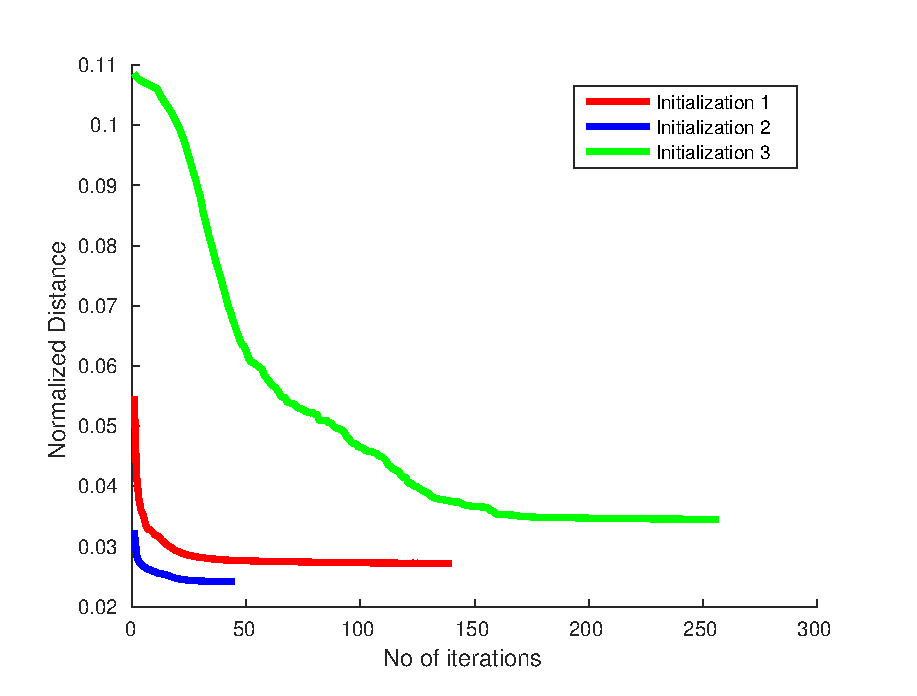
\epsfig{file=images/dist_change_euall.png,  width=0.5\textwidth}
\caption{The convergence of solution for \textbf{EUall} dataset. The number of iterations it took to converge differs for different initializations.}
\end{figure}

\begin{figure*}
\centering
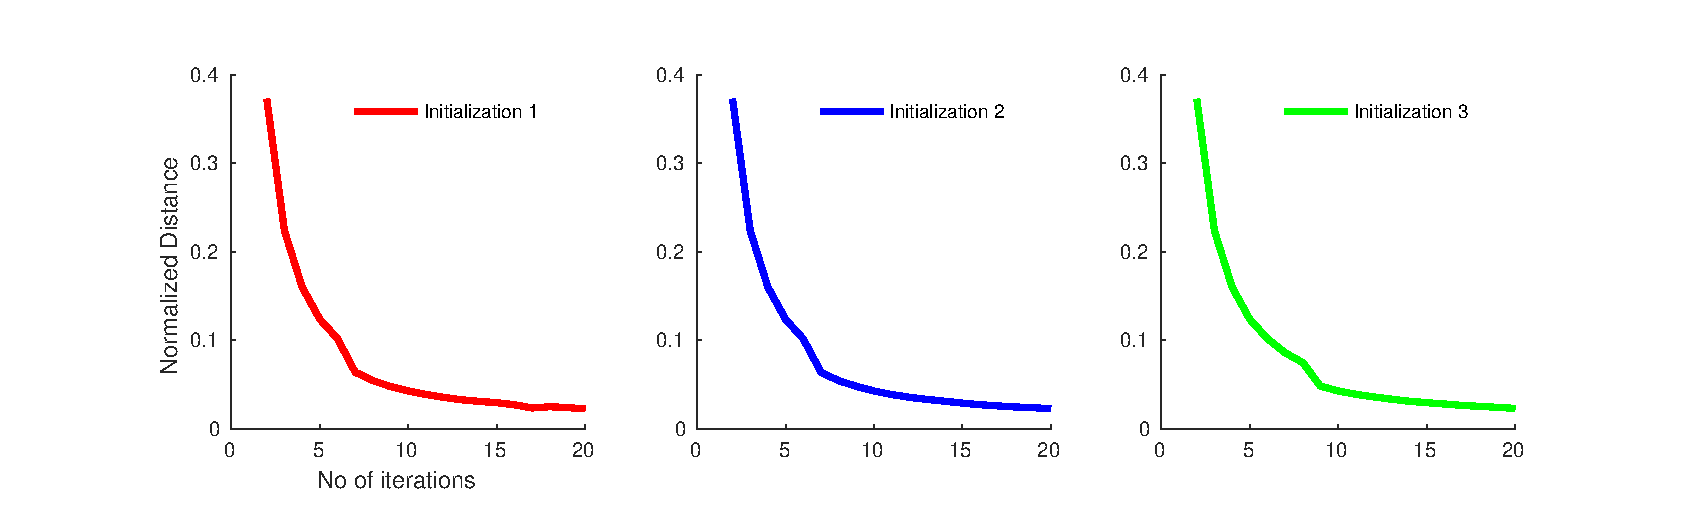
\epsfig{file=images/varying_k_distance.png,height=0.2\textheight, width=\textwidth}
\caption{The normalized distance of \textbf{facebook} dataset for different k ranging from 2 to 20.}
\end{figure*}

\begin{figure*}
\centering
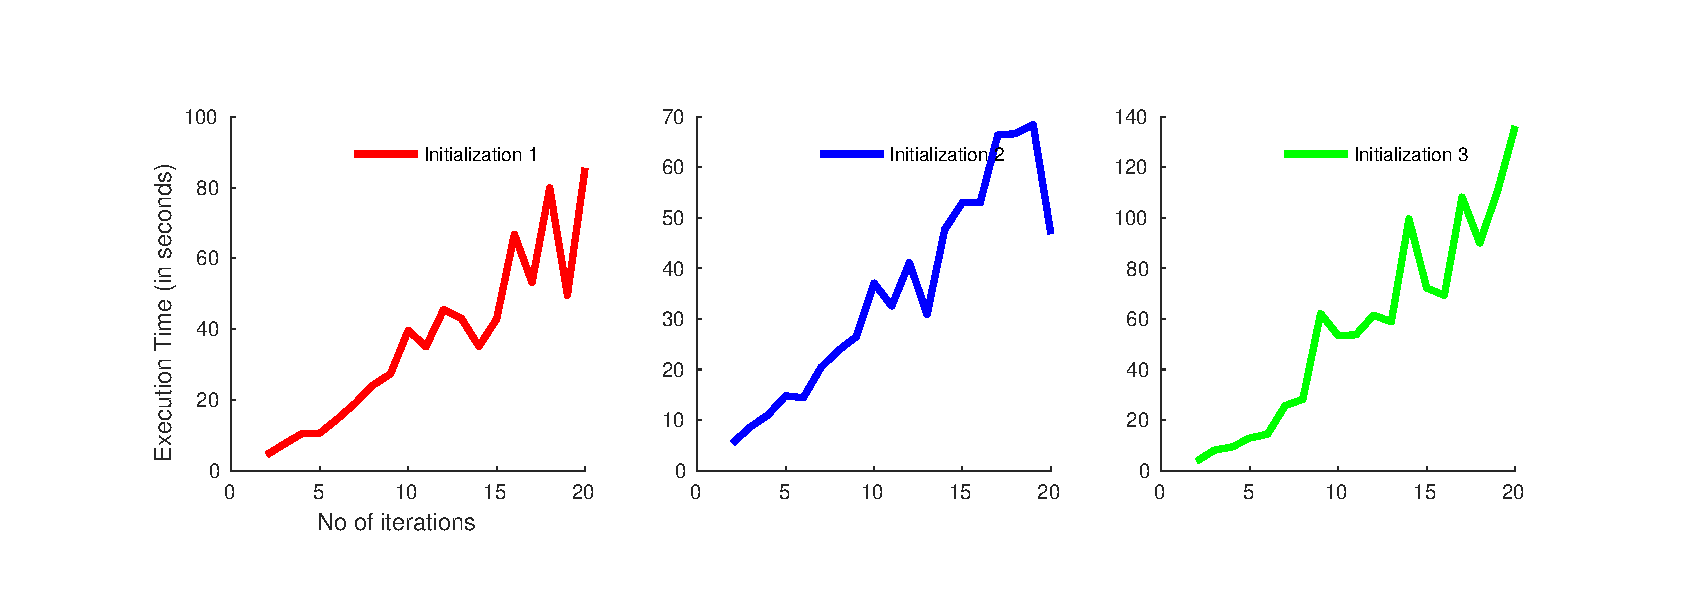
\epsfig{file=images/varying_k_time.png,height=0.2\textheight, width=\textwidth}
\caption{The execution time of \textbf{facebook} dataset for different k ranging from 2 to 20.}
\end{figure*}

\begin{figure}
\begin{tikzpicture}
\begin{axis}[xlabel={iteration $i$}, ylabel= {$\cost{\role_i} / \cost{\role'}$},
    height = 3.5cm,
    width = \columnwidth,
    cycle list name=yaf,
	yticklabel style={/pgf/number format/fixed},
	scaled ticks = false,
    %xmin = 1,
    %ymin = 0.2,
    %ymax = 1,
	ymin = 0.02,
	ytick = {0.02, 0.04, 0.06, 0.08, 0.1},
    xtick = {1, 51, 101, 151, 201, 251},
	legend entries = {\alginitrnd, \alginitdeg, \alginitone, \alginitkm}
    ]

\addplot+[no markers]
    table[x expr = {\coordindex + 1}, y index = 1, header = false]  {images/plot data/euall_init3.log};
\addplot+[no markers]
    table[x expr = {\coordindex + 1}, y index = 1, header = false]  {images/plot data/euall_init1.log};
\addplot+[no markers]
    table[x expr = {\coordindex + 1}, y index = 1, header = false]  {images/plot data/euall_init2.log};
\addplot+[no markers]
    table[x expr = {\coordindex + 1}, y index = 1, header = false]  {images/plot data/euall_init4.log};

\pgfplotsextra{\yafdrawaxis{1}{257}{0.02}{0.11}}
\end{axis}
\end{tikzpicture}
\caption{The convergence of solution for \EUall dataset. The cost of a role assignment $r_i$ at the end of $i$th iteration,
normalized by $\cost{r'}$ such that $r'(v) = 0$, for every $v$, that is, $r'$ assigns the same role to every vertex.}
\end{figure}
\fi
